\documentclass{article}
\usepackage[T1]{fontenc}
\usepackage[utf8]{inputenc}
\usepackage[swedish]{babel}
\usepackage{amsmath, mathtools}
\usepackage{tikz}
\usepackage{titlesec}
\usepackage{lmodern, microtype}
\usepackage{enumitem}

\renewcommand{\vec}[1]{\mathbf{#1}}
\usetikzlibrary{calc}
\titleformat{\section}[runin]{\normalfont\itshape}{\thesection}{1em}{}[:]
\tikzset{
	MyPersp/.style={scale=1.8, x={(-0.8cm,-0.4cm)}, y={(0.8cm,-0.4cm)}, z={(0cm,1cm)}}
}

\author{Axel Forsman}
\title{Stokes sats}

\begin{document}
\maketitle

\begin{center}
	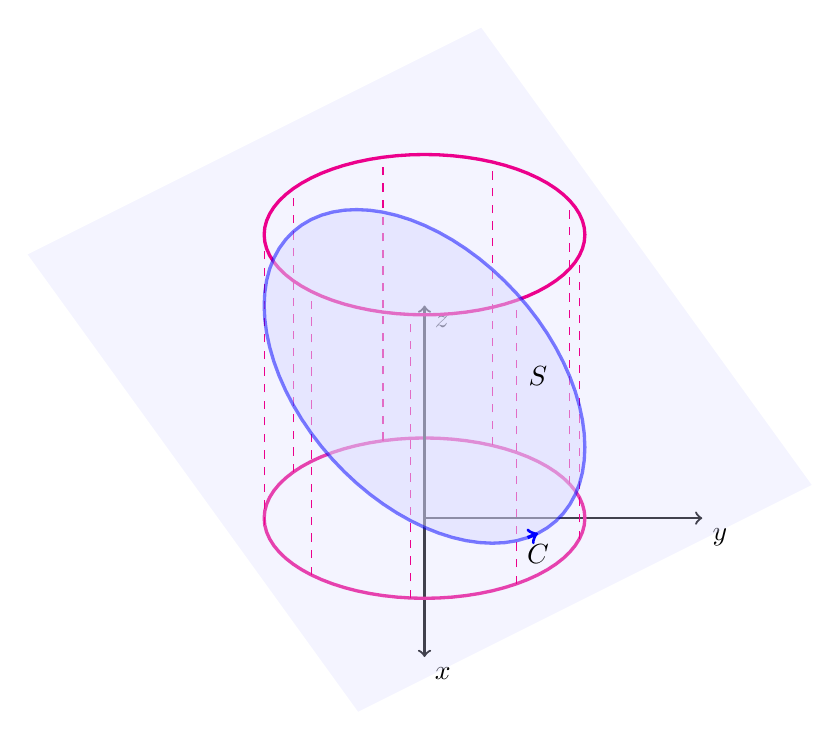
\begin{tikzpicture}[MyPersp]
		\def\h{1} % Height of the ellipse center
		\def\a{35.26}
		\pgfmathparse{\h/tan(\a)}\let\b\pgfmathresult
		\pgfmathparse{sqrt(1/cos(\a)/cos(\a)-1)}\let\c\pgfmathresult % Center Focus distance of the section ellipse

		% Coordinate axes
		\draw[->, thick] (0,0,0) -- ({sqrt(1.5)},{sqrt(1.5)},0) node[below right] {$x$};
		\draw[->, thick] (0,0,0) -- (-{sqrt(1.5)},{sqrt(1.5)},0) node[below right] {$y$};

		\draw[magenta, very thick] (1,0,0) % Lower circle
			\foreach \t in {5,10,...,360}
				{--({cos(\t)},{sin(\t)},0)}--cycle;

		\draw[->, thick] (0,0,0) -- (0,0,1.5) node[below right] {$z$};

		% Draw plane
		\fill[blue!15, opacity=0.3] (2,\b,0) -- (-2,\b,0) -- (-2,-1.5,{(1.5+\b)*tan(\a)})
			-- (2,-1.5,{(1.5+\b)*tan(\a)}) -- cycle;

		\foreach \t in {40,80,...,360} % Generatrices
			\draw[magenta, dashed] ({cos(\t)},{sin(\t)},0) -- ({cos(\t)},{sin(\t)},{2*\h});
		\draw[magenta, very thick] (1,0,{2*\h}) % Upper circle
			\foreach \t in {5,10,...,360}
				{--({cos(\t)},{sin(\t)},{2*\h})}--cycle;

		\fill[blue!15,draw=blue,very thick,opacity=0.5]
			(0,1,{\h-tan(\a)}) % Elliptical section
				\foreach \t in {5,10,...,360}
					{--({sin(\t)},{cos(\t)},{-tan(\a)*cos(\t)+\h})}--cycle;
		\draw[->, blue, very thick] ({sin(5)},{cos(5)},{-tan(\a)*cos(5)+\h}) -- (0,1,{\h-tan(\a)}) node[below, black] (C) {$C$};
		\node at (C |- 0,0,\h) {$S$};
	\end{tikzpicture}
\end{center}

\section*{Problem}
Låt $C$ vara kurvan som ges av skärningen mellan cylindern $x^2 + y^2 = a^2$
och planet $x + y + z = b$ för konstanta $a$ och $b$. \\
Låt $\vec F = y^3 \vec i - x^3 \vec j + z^3 \vec k$.

\begin{enumerate}[label=\alph*)]
	\item Gör en direkt beräkning av kurvintegralen $\oint_C \vec F \cdot d\vec r$
		genom att parametrisera $C$ på lämpligt sätt.
	\item Gör istället beräkningen genom att använda Stokes sats för en lämplig
		yta $S$ vars rand är $C$.
\end{enumerate}

\section*{Lösning}
Byt till cylindriska koordinater $(r, \theta, z)$ så att
$ x = r \cos(\theta), \quad y = r \sin(\theta) $.

\begin{enumerate}[label=\alph*)]
	\item
		\begin{align*}
			x^2 + y^2 = a^2 &\Leftrightarrow r^2 (\cos^2(\theta) + \sin^2(\theta)) = a^2 \\
			&\Leftrightarrow r^2 = a^2 \overset{r \ge 0}{\Leftrightarrow} r = a \\
			x + y + z = b &\Leftrightarrow a \cos(\theta) + a \sin(\theta) + z = b \\
			&\Leftrightarrow z = b - a (\cos(\theta) + \sin(\theta))
		\end{align*}

		Parametriserar $C$ med
		$$ \vec r(\theta) = a \cos(\theta) \vec i + a \sin(\theta) \vec j
			+ (b - a (\cos(\theta) + \sin(\theta))) \vec k, \quad \theta \in [0, 2\pi] $$
		Får att
		\begin{align*}
			I &\coloneqq \oint_C \vec F \cdot d\vec r \\
			&= \int^{2\pi}_0 \overbrace{\vec F(\vec r(\theta))}^{= a^3 \sin^3\theta \vec i - a^3 \cos^3\theta \vec j + (b - a (\cos\theta + \sin\theta))^3 \vec k} \cdot \underbrace{\vec r'(\theta)}_{\rlap{\scriptsize$= -a \sin\theta \vec i + a \cos\theta \vec j + a (\sin\theta - \cos\theta) \vec k$}} \, d\theta \\
			&= -a^4 \underbrace{\int^{2\pi}_0 \sin^4\theta + \cos^4\theta \, d\theta}_{=2 \cdot \frac{3\pi}4} + a \underbrace{\int^{2\pi}_0 (\sin\theta - \cos\theta)(b - a (\cos\theta + \sin\theta))^3 \, d\theta}_{\eqqcolon I_1}
		\end{align*}
		där
		\begin{align*}
			I_1 &= \begin{bmatrix}
				u \coloneqq \cos\theta + \sin\theta, \quad \frac{du}{d\theta} = -\sin\theta + \cos\theta, \\
				\text{$u$ injektiv på delintervallen $\left[0, \frac\pi4\right],
				\left[\frac\pi4, \frac{5\pi}4\right], \left[\frac{5\pi}4, 2\pi\right]$}
			\end{bmatrix} \\
			&= -\int_1^{\sqrt2} (b - au)^3 \, du - \int_{\sqrt2}^{-\sqrt2} (b - au)^3 \, du - \int_{-\sqrt2}^1 (b - au)^3 \, du \\
			&= 0
		\end{align*}

	\item Tag $S$ som ellipsskivan som ges av skärningen, med parametrisering
		$$ \vec r(r, \theta) = r \cos\theta \vec i + r \sin\theta \vec j + (b - r (\cos\theta + \sin\theta)) \vec k, \quad r \le a, \theta \in [0, 2\pi] $$
		Beräknar de ingående värdena:
		\begin{align*}
			\frac{\partial\vec r}{\partial r} \times \frac{\partial\vec r}{\partial\theta} &=
			\begin{bmatrix}
				\frac{\partial \vec r}{\partial r} = \cos\theta \vec i + \sin\theta \vec j - (\cos\theta + \sin\theta) \vec k \\
				\frac{\partial \vec r}{\partial \theta} = -r \sin\theta \vec i + r \cos\theta \vec j - r (\cos\theta - \sin\theta) \vec k
			\end{bmatrix} \\
			&= \begin{pmatrix}
				\sin\theta (-r (\cos\theta - \sin\theta)) + (\cos\theta + \sin\theta) r \cos\theta \\
				-(\cos\theta + \sin\theta) (-r \sin\theta) - \cos\theta (-r (\cos\theta - \sin\theta)) \\
				r \cos\theta \cos\theta + r \sin\theta \sin\theta
			\end{pmatrix} \\
			&= (r, r, r) \\
			\nabla \times \vec F &= \left(\frac{\partial F_z}{\partial y} - \frac{\partial F_y}{\partial z}, \frac{\partial F_x}{\partial z} - \frac{\partial F_z}{\partial x}, \frac{\partial F_y}{\partial x} - \frac{\partial F_x}{\partial y}\right) \\
			&= \left(0, 0, -3x^2 - 3y^2\right)
		\end{align*}
		Väljer vi $\frac{\partial \vec r}{\partial r} \times \frac{\partial \vec r}{\partial\theta}$ som normalen till $S$,
		blir dess rand positivt orienterad.
		Alltså ger Stokes sats
		\begin{align*}
			\oint_C \vec F \cdot d\vec r &= \iint_S \nabla \times \vec F \cdot d\vec S \\
				&= \int_0^a \int^{2\pi}_0 (-3) r^3 \, d\theta dr \\
				&= -\frac{3a^4\pi}2
		\end{align*}
\end{enumerate}
\end{document}
